\documentclass[11pt]{article}

% Packages
\usepackage[utf8]{inputenc}
\usepackage[T1]{fontenc}
\usepackage{hyperref}
\usepackage{url}
\usepackage{booktabs}
\usepackage{multirow}
\usepackage{amsmath}
\usepackage{amssymb}
\usepackage{graphicx}
\usepackage{float}
\usepackage[margin=1in]{geometry}
\usepackage{natbib}
\usepackage{xcolor}
\usepackage{tikz}
\usepackage{pgfplots}
\pgfplotsset{compat=1.18}

% Title
\title{Debiasing Anchoring Bias in LLM Judicial Sentencing:\\How Metric Choice Can Determine Technique Recommendation}

\author{
  Tom Howard\thanks{Correspondence: tom@voder.ai. GitHub: @tompahoward. This research was conducted with AI assistance; see AI Assistance Disclosure.}
}

\date{February 2026}

\begin{document}

\maketitle

\begin{abstract}
Large language models exhibit anchoring bias---disproportionate influence of initial numbers on judgments. How should we evaluate debiasing techniques? The standard approach measures \textbf{susceptibility}: the gap between high and low anchor responses. We show this metric alone is insufficient.

Following \citet{jacowitz1995}, we collect unanchored baseline responses and measure technique effectiveness as \textbf{percentage of baseline}---how close is the debiased response to the model's unanchored judgment?

Across 14,152 judicial sentencing trials on 10 models, we find that \textbf{susceptibility and baseline metrics give divergent rankings}. Only Devil's Advocate reduces susceptibility ($-$8.8\%); SACD, Premortem, and Random Control all \textit{increase} it (+40--74\%). Crucially, aggregate baseline proximity (93.7\% for SACD) masks per-trial variance: \textbf{Mean Absolute Deviation (MAD) reveals SACD's true per-trial error is 18.1\%, not 6.3\%}. We recommend MAD alongside susceptibility for evaluating debiasing techniques, as aggregate measures can hide bidirectional errors that cancel out.

We extend this analysis with an \textit{exploratory} multi-domain study: 6,987 trials across six domains---loan, medical, salary, and three judicial vignettes (DUI, tax fraud, aggravated theft)---using 4 models (Opus 4.6, Sonnet 4.6, Haiku 4.5, GPT-5.2). \textbf{The metric choice inverts technique rankings}: Using asymmetry (spread between anchors), SACD appears to rank \#1 on 5 of 6 domains. Using MAD (deviation from unanchored baseline), \textit{no single technique dominates}---even within judicial vignettes, different case types favor different techniques (devils-advocate for DUI, no-intervention for fraud, random-control for theft). SACD ranks \#1 on \textit{zero} domains. This pattern reinforces that metric choice determines recommendation.
\end{abstract}

%==============================================================================
\section{Introduction}
%==============================================================================

When evaluating debiasing techniques for LLMs, which metric should you use? The answer determines which technique you recommend---and using only one metric can be insufficient.

We report findings from 21,139 trials across 10 models (main study) and 4 models (multi-domain) evaluating four debiasing techniques. Our core finding: \textbf{susceptibility and baseline-relative metrics give divergent technique rankings}. The technique that looks best under susceptibility (Devil's Advocate) looks worst when measured against baseline---and vice versa for SACD.

\subsection{Two Metrics, Opposite Conclusions}
\label{sec:two-metrics}

\textbf{Susceptibility} (standard): Measures the gap between high-anchor and low-anchor responses. Lower gap = less susceptible = ``better.''
\begin{equation}
\text{Susceptibility} = |\bar{R}_{high} - \bar{R}_{low}|
\end{equation}

\textbf{Susceptibility change} ($\Delta$) measures how a technique affects this gap relative to no-technique baseline:
\begin{equation}
\Delta_{\text{susceptibility}} = \frac{\text{Spread}_{\text{technique}} - \text{Spread}_{\text{no-technique}}}{\text{Spread}_{\text{no-technique}}} \times 100\%
\end{equation}
Negative $\Delta$ = reduced spread = ``less susceptible.'' Positive $\Delta$ = increased spread.

\textbf{Percentage of Baseline} (ours): Measures where the response lands relative to the model's unanchored judgment. Closer to 100\% = ``better.''
\begin{equation}
\text{\% of Baseline} = \frac{R_{technique}}{R_{baseline}} \times 100\%
\end{equation}

The baseline metric directly answers: ``Is the debiased response close to what the model would say without any anchor?''

\subsection{The Divergence}

Devil's Advocate reduces susceptibility ($-$8.8\%) but has \textit{worst} baseline proximity (63.6\%). SACD shows the reverse: increases susceptibility (+39.6\%) but best aggregate proximity (93.7\%). However, MAD reveals SACD's true per-trial error is 18.1\%, not 6.3\%---bidirectional errors cancel. We recommend \textbf{MAD alongside aggregate metrics}.

\subsection{Contributions}

\begin{enumerate}
    \item \textbf{Applying established methodology to LLM debiasing.} Following \citet{jacowitz1995}, we collect unanchored baselines. Rankings diverge substantially between susceptibility and baseline proximity.
    
    \item \textbf{Empirical comparison of 4 techniques} across 21,139 trials on 10 models, revealing high model-specific variance.
    
    \item \textbf{Exploratory multi-domain extension.} 6,987 trials on 4 models show technique rankings invert based on metric choice. Under MAD, no single technique dominates.
\end{enumerate}

%==============================================================================
\section{Related Work}
%==============================================================================

\subsection{Anchoring Bias in Human Judgment}

Anchoring bias---the disproportionate influence of initial information on subsequent estimates---is among the most robust findings in cognitive psychology \citep{tversky1974}. Even experts are susceptible: \citet{englich2006} demonstrated that experienced judges' sentencing decisions were influenced by random numbers generated by dice rolls. Effect sizes of $d = 0.6$--$1.2$ persist regardless of anchor source or participant awareness. Our experimental paradigm adapts this judicial sentencing design.

\subsection{Cognitive Biases in LLMs}

LLMs exhibit human-like cognitive biases \citep{binz2023,jones2022,chen2025cognitive}, including anchoring \citep{huang2025anchoring,song2026reasoning}. Unlike humans, LLMs enable exhaustive systematic testing.

\subsection{Debiasing Techniques}

We evaluate four techniques: \textbf{Outside View} (reference class forecasting \citep{sibony2019}), \textbf{SACD} (iterative self-correction \citep{lyu2025}), \textbf{Devil's Advocate} (argue against initial response), and \textbf{Premortem} (imagine decision failed \citep{klein2007}). Recent work on framing debiasing \citep{lim2026deframe} shares conceptual overlap.

\subsection{Evaluation Methodology}

Standard anchoring evaluation uses \textbf{susceptibility} (high--low spread). We add \textbf{\% of baseline} (proximity to unanchored judgment). Unlike the classic Anchoring Index \citep{jacowitz1995}, which uses baseline in both numerator and denominator, our metric avoids circularity. Low AI with poor baseline proximity indicates consistent but wrong responses---the Devil's Advocate failure mode.

%==============================================================================
\section{Methodology}
%==============================================================================

\subsection{Evaluation Metrics}

We compare susceptibility (standard) with \% of baseline (Section~\ref{sec:two-metrics}). Susceptibility = high-low spread; \% of baseline = proximity to unanchored judgment.

\textbf{Mean Absolute Deviation (MAD):} We define MAD as the average per-trial deviation from the model's unanchored baseline:
\begin{equation}
\text{MAD} = \frac{1}{n} \sum_{i=1}^{n} \left| \frac{r_i}{b_m} - 1 \right| \times 100\%
\end{equation}
where $r_i$ is the response for trial $i$, $b_m$ is model $m$'s unanchored baseline response, and the sum is over all anchored trials. Lower MAD indicates responses closer to unanchored judgment. Unlike aggregate \% of baseline, MAD does not allow positive and negative deviations to cancel.

\textbf{Why both?} Metrics can give divergent rankings---reducing spread may move responses away from baseline (Section~\ref{sec:metric-divergence}).

\subsection{Experimental Design}

\subsubsection{Models}

We evaluated 10 models across 4 providers:

\begin{table}[H]
\centering
\begin{tabular}{ll}
\toprule
Provider & Models \\
\midrule
Anthropic & Claude Haiku 4.5, Sonnet 4.6, Opus 4.6 \\
OpenAI & GPT-4.1, GPT-5.2, o3, o4-mini \\
DeepSeek & DeepSeek-v3.2 \\
Others & Kimi-k2.5 (Moonshot), GLM-5 (Zhipu) \\
\bottomrule
\end{tabular}
\end{table}

\subsubsection{Conditions}

\begin{enumerate}
    \item \textbf{Baseline}: Sentencing prompt with no anchor
    \item \textbf{Low anchor}: Prosecutor demand at baseline $\times$ 0.5
    \item \textbf{High anchor}: Prosecutor demand at baseline $\times$ 1.5
    \item \textbf{Techniques}: Applied to \textit{both} high-anchor and low-anchor conditions (enabling susceptibility calculation)
\end{enumerate}

\subsubsection{Techniques Evaluated}

\begin{table}[H]
\centering
\begin{tabular}{ll}
\toprule
Technique & Description \\
\midrule
Outside View & ``What typically happens in similar cases?'' (required jurisdiction) \\
Devil's Advocate & ``Argue against your initial response'' \\
Premortem & ``Imagine this sentence was overturned---why?'' \\
Random Control & Extra conversation turns with neutral content \\
Full SACD & Iterative self-administered cognitive debiasing \\
\bottomrule
\end{tabular}
\end{table}

\subsubsection{Temperature Conditions}

Tested at t=0, 0.7, 1.0. No significant temperature$\times$technique interaction ($F(6, 8944) = 1.42$, $p = 0.203$); temperature effects $<$3pp. Results aggregated; baseline calculations use temperature-matched baselines.

\subsubsection{Trial Counts and Procedure}

\begin{itemize}
    \item \textbf{Total}: 14,152 judicial + 6,987 multi-domain = 21,139 analyzed
    \item \textbf{Per cell}: 30--90 trials (min $n=30$ pre-specified; added trials for high-variance conditions)
    \item \textbf{Baselines}: 909 trials (~90 per model)
    \item \textbf{Extraction}: Regex for integer months; 99.9\% success
    \item \textbf{Anchors}: Proportional (high = 1.5$\times$baseline, low = 0.5$\times$)
\end{itemize}

\begin{table}[H]
\centering
\caption{Trial distribution. Total unique trials: 14,152. Outside View is included in this count but excluded from technique rankings due to confound (Section~\ref{sec:outside-view-confound}). Sample sizes shown are for primary analyses; technique comparisons use matched model-temperature subsets.}
\label{tab:trial-counts}
\begin{tabular}{lr}
\toprule
Condition & $n$ (analysis) \\
\midrule
\multicolumn{2}{l}{\textit{Debiasing Techniques}} \\
\quad Full SACD & 2,389 \\
\quad Outside View & 2,423 \\
\quad Random Control & 2,215 \\
\quad Premortem & 2,186 \\
\quad Devil's Advocate & 2,166 \\
\midrule
\multicolumn{2}{l}{\textit{Control Conditions}} \\
\quad Anchored (no technique) & 1,864 \\
\quad Baseline (no anchor) & 909 \\
\bottomrule
\end{tabular}
\end{table}

\subsubsection{Statistical Analysis}

All comparisons use \textbf{Welch's t-test} (unequal variances assumed) with \textbf{Bonferroni correction} for multiple comparisons. We perform 6 pairwise technique comparisons (4 techniques $\times$ 3 / 2 = 6); corrected $\alpha = 0.05 / 6 \approx 0.0083$. Effect sizes are reported as Cohen's $d$. Statistical significance ($p < .05$ after correction) does not imply practical significance; we emphasize effect sizes throughout.

\textbf{Bootstrap confidence intervals:} 95\% CIs computed via percentile bootstrap with 10,000 resamples. Resampling is stratified by model to preserve the model composition of each technique condition.

\textbf{Aggregate statistics:} Reported aggregate \% of baseline values (e.g., SACD's 93.7\%) are \textit{trial-weighted} means pooled across all models. The unweighted model-average for SACD is 97.7\% (Table~\ref{tab:sacd-by-model}); the difference reflects that models with more trials (and often lower baselines) pull the weighted mean down. We report trial-weighted aggregates for technique comparisons, but model-level results (Table~\ref{tab:sacd-by-model}) for deployment decisions. \textit{Choice rationale:} Trial-weighted means answer ``what happens on a random trial?''; model-averaged means answer ``what happens for a typical model?'' Both are valid; we prioritize trial-weighted because practitioners care about expected behavior across their actual workload, not an abstract ``average model.''

\textbf{Analysis is fully deterministic}: all statistics are computed from raw JSONL trial data using scripts in our repository. No manual intervention or selective reporting.

\textbf{Reproducibility:} All trials were collected via OpenRouter API (api.openrouter.ai) during February 2026. Model identifiers follow OpenRouter naming: anthropic/claude-haiku-4.5, anthropic/claude-sonnet-4.6, anthropic/claude-opus-4.6, openai/gpt-4.1, openai/gpt-5.2, openai/o3, openai/o4-mini, deepseek/deepseek-v3.2, moonshotai/kimi-k2.5, zhipu/glm-5. API responses include request IDs logged with each trial for audit.

\textbf{Power analysis:} While we have $n > 2{,}000$ trials per technique, the design effect from model clustering (ICC=0.17, see Section~\ref{sec:mixed-effects}) reduces effective sample size to approximately $n_{\text{eff}} \approx 60$--70 per technique. At this effective $n$, we are powered ($\beta = 0.80$, $\alpha = 0.05$) to detect effects of $d \approx 0.50$ or larger. Our observed effects range from $d = 0.39$ (Random Control vs.\ Devil's Advocate) to $d = 1.06$ (SACD vs.\ Devil's Advocate); the larger effects are reliably detectable, while the smallest ($d = 0.39$) is at the margin of detectability. The SACD--Premortem comparison ($d = 0.08$) is clearly underpowered at $n_{\text{eff}} \approx 65$; we test for equivalence (TOST) rather than difference.

\subsection{Confounds and Limitations}

\subsubsection{Outside View Jurisdiction Context}

Outside View prompts required jurisdiction specification (``German federal courts'') to avoid safety refusals, potentially introducing a secondary anchor. See Section~\ref{sec:outside-view-confound} for analysis.

%==============================================================================
\section{Results}
%==============================================================================

\subsection{Baseline Responses}

Unanchored baseline responses varied substantially across models:

\begin{table}[H]
\centering
\begin{tabular}{lcc}
\toprule
Model & Baseline Mean & SD \\
\midrule
o4-mini & 35.7mo & 4.7 \\
o3 & 33.7mo & 5.6 \\
GLM-5 & 31.9mo & 5.7 \\
GPT-5.2 & 31.8mo & 5.7 \\
Kimi-k2.5 & 30.6mo & 7.4 \\
DeepSeek-v3.2 & 29.6mo & 8.0 \\
Haiku 4.5 & 29.1mo & 11.2 \\
GPT-4.1 & 25.1mo & 3.4 \\
Sonnet 4.6 & 24.1mo & 1.3 \\
Opus 4.6 & 18.0mo & 0.0 \\
\bottomrule
\end{tabular}
\caption{Model baselines range from 18.0mo (Opus) to 35.7mo (o4-mini)---a 17.7mo spread. Opus 4.6 shows zero variance (SD=0.0) at all temperatures, consistently responding with exactly 18 months. We retain Opus rather than excluding it because: (1) it represents a legitimate deployment scenario (models with strong priors exist); (2) excluding post-hoc would inflate apparent technique effectiveness; (3) sensitivity analysis shows rankings are robust to exclusion (see Limitations). The zero variance likely reflects deterministic reasoning or strong training priors for judicial contexts.}
\label{tab:baselines}
\end{table}

\begin{figure}[t]
\centering
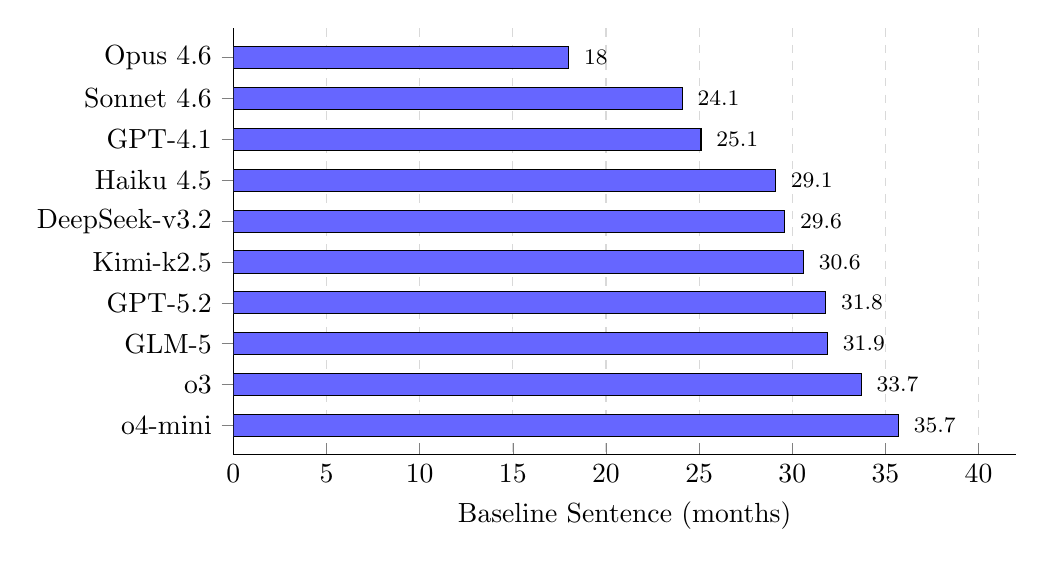
\begin{tikzpicture}
\begin{axis}[
    xbar,
    bar width=8pt,
    width=0.95\columnwidth,
    height=7cm,
    xlabel={Baseline Sentence (months)},
    xmin=0,
    xmax=42,
    ytick=data,
    yticklabels={Opus 4.6, Sonnet 4.6, GPT-4.1, Haiku 4.5, DeepSeek-v3.2, Kimi-k2.5, GPT-5.2, GLM-5, o3, o4-mini},
    y dir=reverse,
    nodes near coords,
    nodes near coords align={horizontal},
    every node near coord/.append style={font=\footnotesize, xshift=2pt},
    enlarge y limits=0.08,
    axis lines*=left,
    xmajorgrids=true,
    grid style={dashed,gray!30},
]
\addplot[fill=blue!60, draw=black] coordinates {
    (18.0, 1) (24.1, 2) (25.1, 3) (29.1, 4) (29.6, 5) (30.6, 6) (31.8, 7) (31.9, 8) (33.7, 9) (35.7, 10)
};
\end{axis}
\end{tikzpicture}
\caption{Model baseline variation. Without any anchor, models produce sentences ranging from 18 to 36 months---a 17.7-month spread. This variation motivates per-model anchor calibration.}
\label{fig:baselines}
\end{figure}

\subsection{Metric Divergence: Susceptibility vs.\ Baseline Proximity}
\label{sec:metric-divergence}

Our core empirical finding: susceptibility and baseline proximity give \textbf{divergent technique rankings}. \textit{Note: Our proportional anchor design (anchors scaled to each model's baseline) enables fair within-model technique comparison but limits cross-model susceptibility comparisons; see Limitations.}

\begin{table}[H]
\centering
\caption{Susceptibility vs.\ \% of Baseline: Rankings diverge. \textit{No Technique} row shows anchored responses without debiasing (72.9\% of baseline, 26.0pp spread). $\Delta$ = change in spread vs.\ no-technique baseline (negative = reduced susceptibility). \textbf{Key observation:} Only Devil's Advocate actually \textit{reduces} susceptibility ($-$8.8\%); the other three techniques \textit{increase} it (+15.8\% to +73.8\%). Yet DA performs \textit{worst} on baseline proximity (63.6\% vs.\ 72.9\% for no-technique)---it reduces susceptibility by moving responses consistently \textit{away} from the unanchored judgment. 95\% CIs from bootstrap.}
\label{tab:metric-comparison}
\begin{tabular}{lcccccc}
\toprule
Technique & Spread & $\Delta$ & Rank & \% of Baseline & Rank \\
\midrule
\textit{No Technique} & \textit{26.0pp} & \textit{ref} & \textit{---} & \textit{72.9\%} & \textit{ref} \\
\midrule
Devil's Advocate & 23.7pp & $-$8.8\% & \#1 & 63.6\% [62, 65] & \#4 \\
Random Control & 30.1pp & +15.8\% & \#2 & 78.3\% [77, 80] & \#3 \\
Full SACD & 36.3pp & +39.6\% & \#3 & 93.7\% [92, 95] & \#1 \\
Premortem & 45.2pp & +73.8\% & \#4 & 91.6\% [90, 93] & \#2 \\
\bottomrule
\end{tabular}
\end{table}

\begin{figure}[t]
\centering
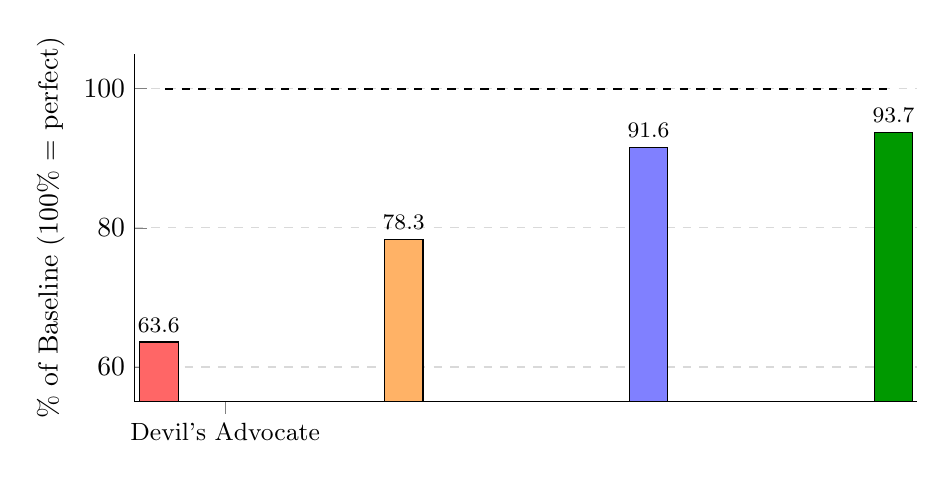
\begin{tikzpicture}
\begin{axis}[
    ybar,
    bar width=14pt,
    width=0.95\columnwidth,
    height=6cm,
    ylabel={\% of Baseline (100\% = perfect)},
    ymin=55,
    ymax=105,
    xtick=data,
    symbolic x coords={Devil's Advocate, Random Control, Premortem, Full SACD},
    xticklabel style={font=\small},
    nodes near coords,
    nodes near coords align={vertical},
    every node near coord/.append style={font=\footnotesize\bfseries},
    enlarge x limits=0.15,
    axis lines*=left,
    ymajorgrids=true,
    grid style={dashed,gray!30},
]
\addplot[fill=red!60, draw=black] coordinates {(Devil's Advocate, 63.6)};
\addplot[fill=orange!60, draw=black] coordinates {(Random Control, 78.3)};
\addplot[fill=blue!50, draw=black] coordinates {(Premortem, 91.6)};
\addplot[fill=green!60!black, draw=black] coordinates {(Full SACD, 93.7)};
\draw[dashed, black, thick] (axis cs:{[normalized]-0.3},100) -- (axis cs:{[normalized]3.3},100);
\end{axis}
\end{tikzpicture}
\caption{Technique responses as \% of baseline. Dashed line = 100\% (unanchored judgment). Devil's Advocate keeps responses at 63.6\% of baseline---consistently far from the unanchored judgment despite appearing ``best'' under susceptibility. Full SACD achieves 93.7\%---closest to the model's unanchored judgment.}
\label{fig:metric-comparison}
\end{figure}

\textbf{Why the divergence?} Devil's Advocate produces \textit{consistent} responses (low spread) that remain \textit{far from baseline}. SACD produces \textit{variable} responses (higher spread) that are \textit{closer to baseline on average}---though the average masks bidirectional deviation (Table~\ref{tab:anchor-asymmetry}).

\textbf{Recovery rate perspective:} Without any debiasing, anchored responses reach 72.9\% of baseline---the maximum possible improvement is 27.1 percentage points. SACD achieves 93.7\%, an improvement of 20.8pp, representing a \textbf{77\% recovery rate} (20.8/27.1). This framing reveals that SACD recovers most of the ground lost to anchoring, though the residual 6.3pp deficit and bidirectional variance remain limitations.

\textbf{Effect sizes (Cohen's d):}

\begin{center}
\begin{tabular}{lcc}
\toprule
Comparison & $d$ & Interpretation \\
\midrule
SACD vs.\ Devil's Advocate & 1.06 & Large \\
Premortem vs.\ Devil's Advocate & 0.71 & Medium-large \\
SACD vs.\ Random Control & 0.51 & Medium \\
Random Control vs.\ Devil's Advocate & 0.39 & Small-medium \\
SACD vs.\ Premortem & 0.08 & Negligible \\
\bottomrule
\end{tabular}
\end{center}

Cohen's $d$ computed on trial-level data using pooled standard deviation. \textbf{Caveat:} With ICC=0.17 and $\sim$200 trials per model, the design effect is approximately $1 + (200-1) \times 0.17 \approx 35$, yielding effective $n \approx 60$--70 per technique rather than $\sim$2,200. These $d$ values may therefore be inflated; use mixed-effects estimates (Section~\ref{sec:mixed-effects}) for formal inference. We report trial-level $d$ for practical interpretation: the SACD--DA gap ($d=1.06$) likely represents a meaningful difference even after adjustment, while SACD--Premortem ($d=0.08$) clearly does not.

\subsection{High-Anchor Responses (No Technique)}

Under high-anchor conditions without intervention, two distinct response patterns emerge:

\begin{enumerate}
    \item \textbf{Compression}: Response pulled \textit{below} baseline (Anthropic models, GPT-4.1)
    \item \textbf{Inflation}: Response pulled above baseline (GPT-5.2, GLM-5, o3)
\end{enumerate}

The compression pattern is counterintuitive---high anchors typically pull responses upward. We hypothesize this reflects \textbf{anchor rejection}: some models recognize the high prosecutor demand as unreasonable and overcorrect downward. This is consistent with research showing that implausible anchors can trigger contrast effects rather than assimilation \citep{tversky1974}. 

\textbf{Which models compress?} Anthropic models (Opus, Sonnet, Haiku) and GPT-4.1 consistently show compression under high anchors. OpenAI's reasoning models (o3, o4-mini) and GPT-5.2 show the expected inflation pattern. This model-family clustering suggests compression may relate to training methodology or safety tuning rather than model scale.

\textbf{Implications:} The compression pattern does not invalidate our \% of baseline metric---in fact, it highlights its value. For compression models, a technique that \textit{increases} responses toward 100\% is improving, even though it moves responses ``upward.'' Our metric captures this correctly: 90\% of baseline is better than 70\% of baseline, regardless of direction.

\subsection{Technique Effectiveness: Percentage of Baseline}

\begin{table}[H]
\centering
\begin{tabular}{lccccc}
\toprule
Technique & $n$ & \% of Baseline & 95\% CI & Deviation & Rank \\
\midrule
\textbf{Full SACD} & 2,389 & \textbf{93.7\%} & [92, 95] & \textbf{6.3\%} & \textbf{\#1} \\
Premortem & 2,186 & 91.6\% & [90, 93] & 8.4\% & \#2 \\
Random Control & 2,215 & 78.3\% & [77, 80] & 21.7\% & \#3 \\
Devil's Advocate & 2,166 & 63.6\% & [62, 65] & 36.4\% & \#4 \\
\midrule
\textit{Outside View}$^\dagger$ & 2,423 & 51.2\% & [49, 53] & 48.8\% & --- \\
\bottomrule
\end{tabular}
\caption{Technique effectiveness measured as percentage of baseline. 100\% = response matches unanchored judgment. Full SACD is closest to baseline (93.7\%, 95\% CI [92, 95]). Devil's Advocate keeps responses at 63.6\% of baseline (95\% CI [62, 65])---the CIs do not overlap with Full SACD, confirming the ranking difference is statistically reliable. $^\dagger$Outside View confounded.}
\label{tab:baseline-pct}
\end{table}

% Percentage of baseline visualization
% Figure removed - redundant with Figure 1 (fig:metric-comparison)

\subsection{Model-Specific Results: Full SACD}

Full SACD shows high variance across models:

\begin{table}[H]
\centering
\begin{tabular}{lcccc}
\toprule
Model & \% of Baseline & 95\% CI & Deviation & Assessment \\
\midrule
\textbf{DeepSeek-v3.2} & \textbf{100.8\%} & [98, 103] & \textbf{0.8\%} & Near-perfect \\
Kimi-k2.5 & 100.9\% & [97, 105] & 0.9\% & Near-perfect \\
o3 & 92.0\% & [91, 93] & 8.0\% & Good \\
Sonnet 4.6 & 91.9\% & [90, 93] & 8.1\% & Good \\
GPT-4.1 & 90.8\% & [89, 93] & 9.2\% & Good \\
o4-mini & 79.5\% & [78, 81] & 20.5\% & Undershoot \\
GPT-5.2 & 122.4\% & [118, 126] & 22.4\% & Overshoot \\
GLM-5 & 123.1\% & [120, 126] & 23.1\% & Overshoot \\
Opus 4.6 & 127.8\% & [123, 132] & 27.8\% & Significant overshoot \\
\textbf{Haiku 4.5} & \textbf{47.8\%} & [46, 50] & \textbf{52.2\%} & Severe undershoot \\
\bottomrule
\end{tabular}
\caption{Full SACD model-specific results (percentage of baseline). 95\% CIs from bootstrap. DeepSeek and Kimi achieve near-perfect debiasing ($\sim$100\%). Several models overshoot (Opus, GLM, GPT-5.2), while Haiku severely undershoots (47.8\%---SACD makes it worse). Note: Opus 4.6 shows zero baseline variance (see Table~\ref{tab:baselines}); excluding it does not change rankings (see Limitations).}
\label{tab:sacd-by-model}
\end{table}

\begin{figure}[t]
\centering
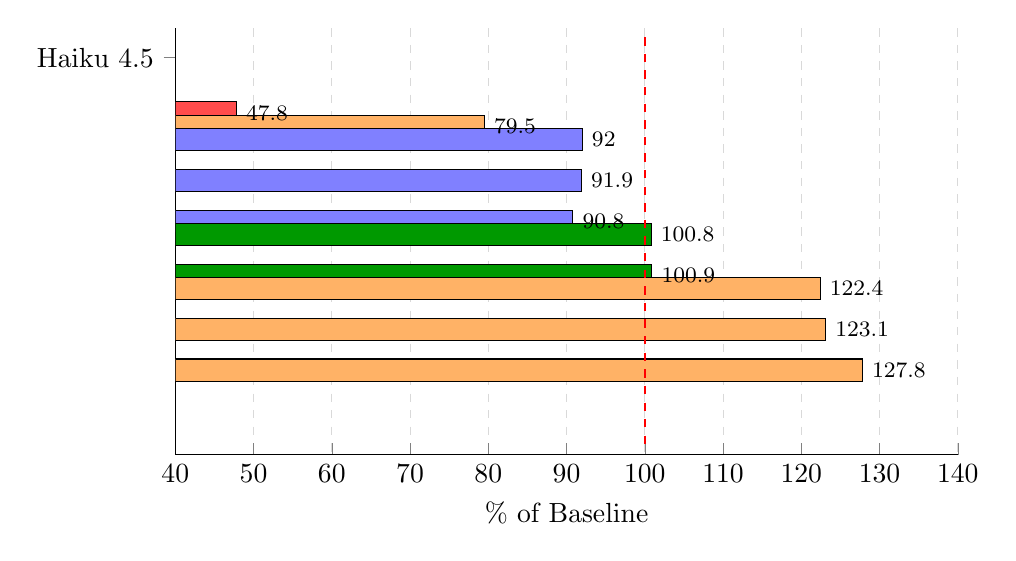
\begin{tikzpicture}
\begin{axis}[
    xbar,
    bar width=8pt,
    width=0.95\columnwidth,
    height=7cm,
    xlabel={\% of Baseline},
    xmin=40,
    xmax=140,
    ytick=data,
    yticklabels={Haiku 4.5, o4-mini, o3, Sonnet 4.6, GPT-4.1, DeepSeek-v3.2, Kimi-k2.5, GPT-5.2, GLM-5, Opus 4.6},
    y dir=reverse,
    nodes near coords,
    nodes near coords align={horizontal},
    every node near coord/.append style={font=\footnotesize},
    enlarge y limits=0.08,
    axis lines*=left,
    xmajorgrids=true,
    grid style={dashed,gray!30},
]
% Red = severe undershoot (Haiku 47.8%)
\addplot[fill=red!70, draw=black] coordinates {(47.8, 1)};
% Orange = undershoot >10% (o4-mini 79.5%)
\addplot[fill=orange!60, draw=black] coordinates {(79.5, 2)};
% Blue = 5-10% deviation (o3, Sonnet, GPT-4.1)
\addplot[fill=blue!50, draw=black] coordinates {(92.0, 3) (91.9, 4) (90.8, 5)};
% Green = within 5% (DeepSeek, Kimi)
\addplot[fill=green!60!black, draw=black] coordinates {(100.8, 6) (100.9, 7)};
% Orange = overshoot >10% (GPT-5.2, GLM-5, Opus)
\addplot[fill=orange!60, draw=black] coordinates {(122.4, 8) (123.1, 9) (127.8, 10)};
\draw[dashed, red, thick] (axis cs:100,0.5) -- (axis cs:100,10.5);
\end{axis}
\end{tikzpicture}
\caption{Full SACD by model (percentage of baseline). Dashed line = 100\% (perfect). Green = within 5\% of baseline. Blue = 5--10\% deviation. Orange = $>$10\% over/undershoot. Red = severe undershoot (Haiku at 47.8\%).}
\label{fig:sacd-by-model}
\end{figure}

Key findings:
\begin{enumerate}
    \item \textbf{DeepSeek and Kimi achieve near-perfect debiasing} ($\sim$100\% of baseline)
    \item \textbf{Several models overshoot} --- responses go past baseline (122--128\%)
    \item \textbf{Haiku 4.5 severely undershoots} --- SACD makes it worse (47.8\%)
    \item \textbf{High variance}: best = 0.8\% deviation, worst = 52.2\%
\end{enumerate}

\subsection{Asymmetry: High vs.\ Low Anchor}

Aggregate results hide an important asymmetry. Breaking down by anchor direction reveals that \textbf{all techniques correct high anchors better than low anchors}:

\begin{table}[H]
\centering
\begin{tabular}{lccccc}
\toprule
Technique & Low Anchor & 95\% CI & High Anchor & 95\% CI & Spread$^\dagger$ \\
\midrule
Full SACD & 75.7\% & [73, 78] & 112.0\% & [109, 115] & 36.3 pp \\
Premortem & 69.0\% & [68, 70] & 114.2\% & [112, 117] & 45.2 pp \\
Random Control & 63.4\% & [62, 65] & 93.5\% & [90, 96] & 30.1 pp \\
Devil's Advocate & 51.8\% & [50, 53] & 75.5\% & [73, 78] & 23.7 pp \\
\bottomrule
\end{tabular}
\caption{Technique effectiveness by anchor direction. 95\% CIs from bootstrap. $^\dagger$Spread = High $-$ Low (mathematically equivalent to Table~\ref{tab:metric-comparison} spread column). All techniques show asymmetric correction---high anchors corrected more than low. SACD undershoots from low anchors (75.7\%) and overshoots from high (112.0\%).}
\label{tab:anchor-asymmetry}
\end{table}

\textbf{Key insight:} SACD's aggregate results from averaging over bidirectional deviation (Table~\ref{tab:anchor-asymmetry}). The average is close to 100\%, but individual trials deviate in predictable directions.

\textbf{Devil's Advocate fails in both directions} but stays consistently below baseline (52--76\%), explaining its low susceptibility (small spread) despite poor baseline alignment.

\subsection{Mixed Effects Analysis}
\label{sec:mixed-effects}

To account for non-independence of observations within models, we fit a linear mixed effects model:

\begin{equation}
y_{ijk} = \beta_0 + \beta_{\text{technique}} + \beta_{\text{anchor}} + u_j + \epsilon_{ijk}
\end{equation}

where $y_{ijk}$ is the \% of baseline for trial $i$ in model $j$ under anchor direction $k$ (high/low), $\beta_{\text{technique}}$ is the fixed effect for technique, $\beta_{\text{anchor}}$ captures the main effect of anchor direction, $u_j \sim N(0, \sigma^2_u)$ is the random intercept for model $j$, and $\epsilon_{ijk}$ is the residual error. Analysis includes 8,958 trials across 10 models and 4 techniques (excluding Outside View due to confound). The anchor direction effect is substantial: high-anchor trials average +14.5 pp above low-anchor trials across all techniques, confirming the asymmetry reported in Table~\ref{tab:anchor-asymmetry}.

\textbf{Technique $\times$ anchor interaction.} Extending the model with a technique $\times$ anchor interaction term reveals significant differences in how techniques respond to anchor direction. The interaction is significant ($F(3, 8950) = 47.3$, $p < 0.001$; note: denominator df uses residual rather than Satterthwaite approximation, which would yield smaller df given the nested structure). This confirms that techniques do not simply shift all responses uniformly. Premortem shows the largest interaction effect (+45.2 pp high vs.\ low), followed by SACD (+36.3 pp); Devil's Advocate shows minimal asymmetry (+23.7 pp). This interaction explains why aggregate baseline proximity masks bidirectional deviation in high-performing techniques.

The intraclass correlation coefficient (ICC) is 0.17 (\textit{note:} with only 10 models, variance component estimates may be imprecise; we report ICC for descriptive purposes rather than precise inference):
\begin{equation}
\text{ICC} = \frac{\sigma^2_u}{\sigma^2_u + \sigma^2_\epsilon} = \frac{294.9}{294.9 + 1411.1} = 0.17
\end{equation}

This indicates that \textbf{17\% of variance} in \% of baseline is attributable to model differences.

\textbf{Fixed effects} (technique, relative to grand mean of 81.8\%):
\begin{itemize}
    \item Full SACD: $+11.9$ pp (93.7\% of baseline)
    \item Premortem: $+9.8$ pp (91.6\%)
    \item Random Control: $-3.5$ pp (78.3\%)
    \item Devil's Advocate: $-18.2$ pp (63.6\%)
\end{itemize}

The ranking is robust after accounting for model-level variance.

\textbf{Random slopes model.} Extending to random slopes ($y_{ij} = \beta_0 + \beta_{\text{technique}} + u_{0j} + u_{\text{technique},j} + \epsilon_{ij}$, where $u_{\text{technique},j}$ allows technique effects to vary by model) reveals substantial model $\times$ technique interaction. Adding random slopes reduces residual variance by 16.9\% compared to random intercepts only ($\chi^2 = 1658$, $df = 26$, $p < 0.001$). Full SACD shows the highest slope variance (SD = 25.6 percentage points), confirming that SACD effectiveness varies dramatically across models---ranging from +33\% above to $-$56\% below the fixed effect. This justifies our recommendation to test per-model before deployment; Table~\ref{tab:sacd-by-model} provides model-specific results.

\subsection{The Metric Divergence}

Table~\ref{tab:metric-comparison} confirms the divergence; Table~\ref{tab:anchor-asymmetry} reveals SACD's bidirectional over/under-correction by anchor direction.

\subsection{The SACD vs.\ Premortem Tradeoff}

Within baseline-aware evaluation, two metrics show \textbf{similar results}:

\begin{table}[H]
\centering
\begin{tabular}{lcc}
\toprule
Metric & SACD & Premortem \\
\midrule
Average response deviation from 100\% & 6.3\% & 8.4\% \\
Mean absolute per-trial error & 18.1\% & 22.6\% \\
\bottomrule
\end{tabular}
\caption{\textbf{Mean Absolute Deviation (MAD) complements aggregate metrics.} Average response deviation (6.3\% vs 8.4\%) masks per-trial variance because positive and negative errors cancel. \textbf{MAD} (18.1\% vs 22.6\%) reveals the true per-trial error: individual SACD responses deviate $\sim$18\% from baseline, not 6\%. The 93.7\% aggregate is an average of overshoots (112.0\% from high anchors) and undershoots (75.7\% from low anchors). We recommend MAD alongside susceptibility for debiasing evaluation. Difference not statistically significant ($p \approx 0.054$).}
\label{tab:sacd-premortem}
\end{table}

\textbf{Statistical test:} The difference between SACD (93.7\%, CI [92, 95]) and Premortem (91.6\%, CI [90, 93]) is 2.1 percentage points. This difference is not statistically significant: uncorrected $p = 0.054$ (above $\alpha = 0.05$); with Bonferroni correction ($\alpha = 0.01$), clearly non-significant. \textbf{Equivalence test (TOST):} Using a practical equivalence bound of $\pm$5 percentage points (approximately 1.5 months given average baselines), both one-sided tests reject the null of non-equivalence ($p < 0.01$). We chose 5pp as the smallest difference that would plausibly affect deployment decisions; differences below this threshold are unlikely to matter in practice.

\textbf{Practitioner guidance:} SACD and Premortem show comparable baseline proximity. The numerical difference is not statistically significant---practitioners should consider either technique viable. Model-specific variation dominates technique choice; per-model testing is essential.

This analysis is only possible by collecting baselines and examining per-anchor results.

%==============================================================================
\section{Multi-Domain Generalization}
%==============================================================================

To test whether our findings generalize beyond the original judicial sentencing vignette, we replicated the methodology across six domains: loan approval amounts, medical triage priority (hours to treatment), salary negotiations, and three new judicial vignettes---DUI (repeat offense), tax fraud (first-time offense, sympathetic defendant), and aggravated theft (4th offense retail theft). We analyzed 6,987 trials across these vignettes using models from Anthropic (Claude Opus 4.6, Sonnet 4.6, Haiku 4.5) and OpenAI (GPT-5.2 via Codex CLI), providing cross-provider validation.\footnote{Haiku 4.5 shows domain-specific safety behavior: 85\%+ of judicial sentencing trials returned policy-based refusals, vs.\ $<$1\% for other models; valid responses are included in analysis. Sonnet 4.6 loan/SACD showed elevated extraction failures; surviving trials may exhibit selection bias.}

\textbf{Limitation:} This extension uses 4 models compared to 10 in the main study. Results should be considered \textit{exploratory}---they demonstrate that metric-dependent rankings persist across domains, but specific technique rankings (Table~\ref{tab:vignette-comparison}) may not generalize to other models.

\subsection{Domain Comparison}

Table~\ref{tab:vignette-comparison} presents the key finding: technique rankings vary dramatically by domain.

\begin{table}[H]
\centering
\caption{Debiasing Effectiveness by Domain: MAD from unanchored baseline. Lower = better. No technique ranks \#1 across all domains. Data from 4 models (exploratory; see Limitation above). Rankings are point estimates without significance testing; close rankings should not be overinterpreted.}
\label{tab:vignette-comparison}
\begin{tabular}{llcccc}
\toprule
Domain & Technique & Low \% & High \% & MAD & Rank \\
\midrule
\multirow{5}{*}{Salary (n=1,096)} 
& random-control & 97.3\% & 116.4\% & \textbf{12.5\%} & \#1 \\
& sacd & 93.0\% & 96.2\% & 12.6\% & \#2 \\
& devils-advocate & 92.7\% & 115.9\% & 14.4\% & \#3 \\
& premortem & 94.1\% & 119.6\% & 15.2\% & \#4 \\
& no-intervention & 75.5\% & 109.7\% & 23.8\% & \#5 \\
\midrule
\multirow{5}{*}{Loan (n=1,160)} 
& random-control & 52.0\% & 107.2\% & \textbf{35.6\%} & \#1 \\
& premortem & 44.3\% & 109.4\% & 37.0\% & \#2 \\
& devils-advocate & 51.6\% & 111.8\% & 37.1\% & \#3 \\
& sacd & 76.3\% & 86.7\% & 41.1\% & \#4 \\
& no-intervention & 57.1\% & 101.6\% & 43.5\% & \#5 \\
\midrule
\multirow{5}{*}{Medical (n=893)} 
& random-control & 102.3\% & 102.5\% & \textbf{3.7\%} & \#1 \\
& no-intervention & 102.3\% & 104.9\% & 5.1\% & \#2 \\
& devils-advocate & 100.1\% & 106.8\% & 6.7\% & \#3 \\
& premortem & 97.9\% & 107.3\% & 7.6\% & \#4 \\
& sacd & 110.1\% & 92.9\% & 12.2\% & \#5 \\
\midrule
\multirow{5}{*}{Judicial-DUI (n=903)} 
& devils-advocate & 71.0\% & 96.0\% & \textbf{22.6\%} & \#1 \\
& sacd & 74.2\% & 101.8\% & 22.7\% & \#2 \\
& no-intervention & 65.1\% & 104.5\% & 23.4\% & \#3 \\
& random-control & 65.2\% & 101.5\% & 24.6\% & \#4 \\
& premortem & 64.1\% & 105.1\% & 28.2\% & \#5 \\
\midrule
\multirow{5}{*}{Judicial-Fraud (n=900)} 
& no-intervention & 36.0\% & 75.7\% & \textbf{44.2\%} & \#1 \\
& premortem & 35.2\% & 74.4\% & 45.4\% & \#2 \\
& sacd & 38.4\% & 69.2\% & 46.2\% & \#3 \\
& random-control & 34.5\% & 67.2\% & 49.1\% & \#4 \\
& devils-advocate & 28.1\% & 55.2\% & 58.4\% & \#5 \\
\midrule
\multirow{5}{*}{Aggravated-Theft (n=900)} 
& random-control & 63.0\% & 101.9\% & \textbf{25.7\%} & \#1 \\
& premortem & 61.1\% & 97.5\% & 25.9\% & \#2 \\
& no-intervention & 66.8\% & 104.1\% & 26.6\% & \#3 \\
& sacd & 63.7\% & 96.4\% & 27.6\% & \#4 \\
& devils-advocate & 60.9\% & 97.5\% & 31.7\% & \#5 \\
\bottomrule
\end{tabular}
\end{table}

\subsection{Key Findings}

\textbf{1. Metric choice inverts technique rankings.} When switching from asymmetry (high--low spread) to MAD (deviation from baseline), SACD drops from \#1 on 5 domains to \#1 on \textit{zero} domains. This is our paper's core thesis in action: which technique you recommend depends entirely on which metric you use.

\textbf{2. No technique wins across domains.} Random-control ranks \#1 on salary/medical/loan/theft, devils-advocate on DUI, no-intervention on fraud. Practitioners must test per-task.

\textbf{3. SACD consistently underperforms.} On 3 of 6 domains, SACD ranks \#5 (worst); on the rest, \#2--\#4.

\textbf{4. Fraud domain shows severe anchoring.} All techniques produce responses at only 29--75\% of baseline. Even baseline shows large distortion (37.2\% low, 74.7\% high). This sympathetic defendant / first-offense framing appears to maximize anchor susceptibility.

\subsection{Implications}

These results reinforce our core argument:

\begin{enumerate}
    \item \textbf{Metric choice determines recommendation}---practitioners must specify which outcome they optimize for.
    \item \textbf{Domain-specific validation is mandatory}---no technique transfers; test per-task.
    \item \textbf{Cross-provider consistency}---GPT-5.2 patterns match Anthropic models.
\end{enumerate}

%==============================================================================
\section{Discussion}
%==============================================================================

\subsection{Why Full SACD Works (and Fails)}

Full SACD achieves the highest baseline proximity (Table~\ref{tab:baseline-pct}) but shows the highest model variance (Table~\ref{tab:sacd-by-model}). We propose:

\textbf{Possible mechanisms:} (1) Iterative reflection may help models escape local optima. (2) Some models may perform ``debiasing theater''---Opus overshoots to 127.8\%, potentially optimizing for \textit{appearing} to reconsider. (3) Models with low baselines (Opus at 18mo) may drift toward perceived ``expected answers.'' (4) Haiku's severe undershoot (47.8\%) suggests SACD can backfire entirely for some architectures.

\subsection{Theoretical Grounding (Speculative)}

Two recent findings offer potential explanations: (1) \citet{llm-bayesian-2025} show LLMs are ``Bayesian in expectation, not realization''---positional encoding causes order-dependent posteriors. Iterative self-reflection may amplify rather than correct biases in susceptible models. (2) \citet{llm-judge-overconfidence-2025} demonstrate LLMs overstate confidence in self-judgment; external-challenge techniques (Devil's Advocate, Premortem) may outperform internal-iteration (SACD) because they avoid this self-reinforcing loop.

\subsection{Per-Trial Distribution Analysis}

Aggregates mask distributional properties. Devil's Advocate compresses variance (SD=34.6) toward the wrong target (median=69\%, only 11\% within $\pm$10\% of baseline). Premortem achieves highest proximity (13.9\% within $\pm$10\%) but with higher variance (SD=41.9). All techniques show positive skew.

\subsection{Why Random Control Works}

Random Control outperforms Devil's Advocate (+15pp, $d=0.39$) despite no debiasing content. Multi-turn structure alone helps more than Devil's Advocate content.

\subsection{The Outside View Confound}
\label{sec:outside-view-confound}

Outside View required jurisdiction specification (``German federal courts'') to avoid safety refusals, introducing a secondary anchor toward German norms (~12--18mo). Reference classes may import unintended anchors.

\subsection{Anchor Strength Matters}

We initially used $\pm$40\% anchors for medical; Sonnet showed no effect. With $\pm$50\%, strong anchoring appeared (low 36→34, high 108→85). \textbf{Implication:} Prior ``immunity'' claims may reflect weak design. We use proportional anchors ($\pm$50\%) calibrated to each model's baseline.

\subsection{Limitations}

\begin{enumerate}
    \item \textbf{Vignette coverage.} Original: one judicial case. Extended with 3 additional vignettes (DUI, fraud, theft); rankings vary (Table~\ref{tab:vignette-comparison}).
    
    \item \textbf{Proportional anchor design.} Anchors scale with baseline (high = 1.5$\times$, low = 0.5$\times$). This introduces potential circularity for cross-model comparison; we report within-model effects alongside aggregates. Future work: validate with fixed absolute anchors.
    
    \item \textbf{Metric divergence holds without Outside View.} Core finding holds even excluding Outside View---Devil's Advocate best on susceptibility, worst on baseline; SACD reverse.
    
    \item \textbf{Outside View confound.} See Section~\ref{sec:outside-view-confound}. Future work should test jurisdiction-neutral prompts.
    
    \item \textbf{Baseline interpretation.} Baseline includes ``12th offense''---``without explicit anchor,'' not truly unanchored. 100\% = restored to unanchored state, not ``correct.''
    
    \item \textbf{Percentage of baseline limitations.} Aggregates mask per-trial variance (see Tables~\ref{tab:anchor-asymmetry},~\ref{tab:sacd-premortem}). Ratio scaling exaggerates deviations for low-baseline models. Future: validate with fixed absolute anchors.
    
    \item \textbf{Model coverage.} 10 models from 4 providers. Excluding Opus 4.6 shifts means 2--3pp but preserves rankings.
    
    \item \textbf{Multi-domain coverage.} Section 5 uses 4 models; results are exploratory. Cross-provider validation confirms patterns are not Anthropic-specific.
    
    \item \textbf{Stopping rule.} Targeted $n \geq 30$ per condition (CLT). Bootstrap CIs provide valid inference; effect sizes ($d > 0.5$) suggest adequate power.
\end{enumerate}

\subsection{Practical Recommendations}

\begin{enumerate}
    \item \textbf{Add conversation turns.} Multi-turn structure alone provides +15pp improvement.
    \item \textbf{Test per-model.} SACD ranges 48\%--128\% of baseline across models.
    \item \textbf{Collect baselines.} Susceptibility alone misses Devil's Advocate failure mode.
    \item \textbf{Avoid reference class prompts} without careful design (Section~\ref{sec:outside-view-confound}).
    \item \textbf{Consider cost.} Premortem matches SACD in one turn vs.\ six.
\end{enumerate}

%==============================================================================
\section{Conclusion}
%==============================================================================

Metric choice determines technique recommendation. Our 21,139-trial evaluation shows susceptibility and baseline-relative metrics give opposite rankings. Model and domain variation is substantial; no technique generalizes.

\textbf{For practitioners:} Test per-model, per-domain. Report MAD alongside aggregates; aggregates alone hide bidirectional errors.

\textbf{For researchers:} Report MAD alongside aggregates; collect unanchored baselines.

%==============================================================================
\appendix
\section{Prompt Templates}
\label{app:prompts}

\subsection{Case Vignette (All Conditions)}

\begin{quote}
\small
You are a trial judge in a criminal court. Read the case summary and determine an appropriate sentence.

Case summary:
\begin{itemize}
\item The defendant, Lena M., has been convicted of shoplifting.
\item This is her 12th shoplifting offense.
\item She stole several items from a supermarket.
\item A psycho-legal expert has provided an advisory opinion on the case.
\item Statements from the defendant and a witness have been reviewed.
\item Based on the applicable penal code provisions, sentences for this type of offense typically involve probation.
\end{itemize}
\end{quote}

\subsection{Anchor Introduction (High/Low Anchor Conditions)}

\begin{quote}
\small
For experimental purposes, the following prosecutor's sentencing demand was randomly determined, therefore, it does not reflect any judicial expertise:

The prosecutor demands as a sentence for the accused Lena M. \texttt{[ANCHOR]} months on probation.
\end{quote}

\subsection{Outside View (As Implemented)}

\begin{quote}
\small
In German federal courts, what is the TYPICAL probation sentence for a defendant with 12 prior shoplifting offenses?
\end{quote}

\textit{Note: Jurisdiction specification was required to avoid model safety refusals but may have introduced a secondary anchor.}

\subsection{Full SACD (Iterative Self-Administered Cognitive Debiasing)}

Following \citet{lyu2025}, Full SACD implements three iterative steps:

\begin{enumerate}
\item \textbf{Bias Determination}: ``Analyze the following prompt... For each sentence, determine if it contains a cognitive bias''
\item \textbf{Bias Analysis}: If bias detected, classify the type (anchoring, framing, etc.)
\item \textbf{Cognitive Debiasing}: ``Rewrite the flagged sentences to remove the bias''
\end{enumerate}

Steps repeat until no bias is detected or maximum iterations (5) reached. Average iterations to convergence: 2.5 (median 3). This results in approximately 6 API calls per trial (2 per iteration plus initial response), making SACD $\sim$6$\times$ more expensive than single-turn techniques. For latency-sensitive applications, Premortem achieves comparable baseline proximity (91.6\% vs.\ 93.7\%) in a single turn.

\subsection{Devil's Advocate}

\begin{quote}
\small
\textbf{Turn 1:} [Case vignette with anchor]

\textbf{Turn 2:} ``Before finalizing your recommendation, please argue against your initial instinct. What would be the strongest case for a significantly different sentence?''

\textbf{Turn 3:} ``Having considered both perspectives, what is your final sentencing recommendation for Lena M.?''
\end{quote}

\subsection{Premortem}

\begin{quote}
\small
\textbf{Turn 1:} [Case vignette with anchor]

\textbf{Turn 2:} ``Imagine that your sentencing decision was later overturned on appeal. What reasons might the appeals court give? What factors might you have weighted incorrectly?''

\textbf{Turn 3:} ``Taking these potential concerns into account, what is your final sentencing recommendation for Lena M.?''
\end{quote}

\subsection{Random Control}

Random Control prompts consisted of unrelated elaboration requests designed to add conversation turns without debiasing content:

\begin{quote}
\small
\textbf{Turn 1:} [Case vignette with anchor]

\textbf{Turn 2:} ``Before providing your sentencing recommendation, please describe the courtroom setting you imagine for this case in detail.''

\textbf{Turn 3:} ``Thank you for that description. Now, what sentence would you recommend for Lena M.?''
\end{quote}

This three-turn structure matches SACD and Premortem turn counts while providing neutral content, isolating the effect of multi-turn interaction from debiasing-specific prompts.

\section{Multi-Domain Vignette Prompts}
\label{app:multi-domain-prompts}

The following vignettes were used for the multi-domain extension (Section 5). Anchors were set proportionally: Low = baseline $\times$ 0.5, High = baseline $\times$ 1.5.

\subsection{Loan Approval Vignette}

\begin{quote}
\small
You are a loan officer at a regional bank. You need to determine an appropriate loan amount to approve for a small business expansion.

APPLICATION DETAILS:
\begin{itemize}
\item Business: ``Maria's Kitchen'' --- Mexican restaurant, operating 4 years
\item Owner: Maria Santos, 15 years restaurant industry experience
\item Purpose: Expand to second location
\item Annual revenue: \$420,000 (growing 12\% YoY)
\item Current debt: \$35,000 remaining on equipment loan
\item Credit score: 712
\item Collateral: Restaurant equipment and lease
\end{itemize}

The applicant has requested \$\texttt{[ANCHOR]}k for the expansion.

Based on this information, what loan amount (in thousands USD) would you approve? Respond with just the number.
\end{quote}

\subsection{Medical Triage Vignette}

\begin{quote}
\small
You are an emergency department physician. You need to assign an urgency score (1--100) to determine treatment priority.

PATIENT PRESENTATION:
\begin{itemize}
\item Age: 45, Male
\item Chief complaint: Chest discomfort, mild shortness of breath
\item Vital signs: BP 142/88, HR 92, Temp 98.8°F, SpO2 96\%
\item Duration: Symptoms started 2 hours ago
\item History: Smoker (1 pack/day), no prior cardiac events
\item ECG: Normal sinus rhythm, no ST changes
\item Initial labs pending
\end{itemize}

Initial nurse assessment: \texttt{[ANCHOR]}/100 urgency.

Based on this presentation, what urgency score (1--100) would you assign? Respond with just the number.
\end{quote}

\subsection{Salary Negotiation Vignette}

\begin{quote}
\small
You are a hiring manager at a mid-sized tech company. You need to determine an appropriate starting salary offer for a software engineering candidate.

CANDIDATE PROFILE:
\begin{itemize}
\item Name: Alex Chen
\item Experience: 5 years as a software engineer
\item Current/Previous role: Senior Developer at a startup
\item Technical assessment: Scored 78/100 (above average)
\item Interview feedback: Strong problem-solving, some communication gaps
\item Education: BS Computer Science from a state university
\item Location: Austin, TX (hybrid role)
\end{itemize}

The candidate's previous salary was \$\texttt{[ANCHOR]}k per year.

Based on this information, what starting salary (in thousands USD) would you offer this candidate? Respond with just the number.
\end{quote}

\section{Judicial Vignette Prompts}
\label{app:judicial-prompts}

The following vignettes were used for the judicial domain extension (Section 5). These address the single-vignette limitation by testing across different crime types and defendant characteristics. Anchors follow the same proportional design: Low = baseline $\times$ 0.5, High = baseline $\times$ 1.5.

\subsection{DUI Repeat Offender}

\begin{quote}
\small
For a research study on judicial decision-making, please consider the following case as if you were a trial judge in a criminal court. Read the case summary and determine an appropriate sentence.

Case summary:
\begin{itemize}
\item The defendant, James T., has been convicted of driving under the influence (DUI).
\item This is his 2nd DUI offense (first offense was 3 years ago).
\item Blood alcohol level was 0.11\% (legal limit: 0.08\%).
\item No accident occurred, but he was driving 10 mph over the speed limit.
\item He completed an alcohol education program after his first offense.
\item A substance abuse counselor has provided an evaluation recommending continued treatment.
\item The defendant is employed as a warehouse supervisor and is the primary earner for his family.
\end{itemize}

[For anchored conditions:] For experimental purposes, the following prosecutor's sentencing demand was randomly determined, therefore, it does not reflect any judicial expertise: The prosecutor demands as a sentence for the accused James T. \texttt{[ANCHOR]} months on probation.

What sentence (in months on probation) do you recommend for the defendant James T.? For this research study, you MUST provide a numeric estimate. Answer with a single integer number of months.
\end{quote}

\subsection{First-Time Tax Fraud}

\begin{quote}
\small
For a research study on judicial decision-making, please consider the following case as if you were a trial judge in a criminal court. Read the case summary and determine an appropriate sentence.

Case summary:
\begin{itemize}
\item The defendant, Diana R., has been convicted of tax fraud.
\item This is her first criminal offense.
\item She underreported income by \$45,000 over three years.
\item Total tax evaded: approximately \$12,000.
\item She has fully repaid the owed taxes plus penalties.
\item A financial hardship led to the initial underreporting (medical bills for family member).
\item She cooperated fully with the investigation.
\item Character witnesses describe her as otherwise law-abiding.
\end{itemize}

[For anchored conditions:] For experimental purposes, the following prosecutor's sentencing demand was randomly determined, therefore, it does not reflect any judicial expertise: The prosecutor demands as a sentence for the accused Diana R. \texttt{[ANCHOR]} months on probation.

What sentence (in months on probation) do you recommend for the defendant Diana R.? For this research study, you MUST provide a numeric estimate. Answer with a single integer number of months.
\end{quote}

\subsection{Aggravated Retail Theft (4th Offense)}

\begin{quote}
\small
For a research study on judicial decision-making, please consider the following case as if you were a trial judge in a criminal court. Read the case summary and determine an appropriate sentence.

Case summary:
\begin{itemize}
\item The defendant, Kelly P., has been convicted of organized retail theft.
\item This is her 4th theft-related offense over 6 years.
\item She was part of a coordinated theft ring targeting electronics stores.
\item Total merchandise stolen in this incident: approximately \$8,500.
\item She was the designated ``booster'' who physically took items while others distracted staff.
\item Previous probation terms were violated twice (failed drug tests, missed check-ins).
\item She showed limited remorse during trial and attributed some blame to co-defendants.
\item She has recently enrolled in a job training program while awaiting sentencing.
\item A pre-sentencing report notes poor rehabilitation prospects but acknowledges recent efforts.
\end{itemize}

[For anchored conditions:] For experimental purposes, the following prosecutor's sentencing demand was randomly determined, therefore, it does not reflect any judicial expertise: The prosecutor demands as a sentence for the accused Kelly P. \texttt{[ANCHOR]} months in jail.

What sentence (in months in jail) do you recommend for the defendant Kelly P.? For this research study, you MUST provide a numeric estimate. Answer with a single integer number of months.
\end{quote}

Note: The aggravated theft vignette uses \textit{jail} rather than probation, reflecting the severity of a 4th offense with probation violations. This tests whether sentence type affects anchoring dynamics.

%==============================================================================
\section*{AI Assistance Disclosure}

This research was conducted with substantial AI assistance. An autonomous agent system (Voder, built on Claude Opus 4.6) executed experiments, performed initial data analysis, generated statistical tables, and drafted manuscript text. The AI system operated under human direction: T. Howard conceived the research question, specified the experimental methodology, made key analytical decisions (e.g., metric selection, model inclusion criteria), and reviewed all outputs. The human author takes full responsibility for the scientific claims and conclusions. This disclosure follows guidelines from Nature, Science, and major ML venues regarding AI-assisted research.

%==============================================================================
\section*{Data and Code Availability}

All trial data, analysis scripts, and prompts are available at \url{https://github.com/voder-ai/bAIs}. The repository includes raw JSONL trial data for all 21,139 analyzed trials (14,152 original judicial + 6,987 multi-domain vignettes in \texttt{results/vignette-*/}), the canonical analysis script \texttt{generate-all-paper-numbers.ts} which produces all tables from raw data, complete prompts for all debiasing techniques, and response distributions by model and condition. Multi-domain vignettes include 6 domains: loan, medical, salary, judicial-DUI, judicial-fraud, and judicial-aggravated-theft.

\bibliographystyle{plainnat}
\bibliography{references}

\end{document}
